% Appendix C: Detailed per-partition results

\subsection{$K_{\mathrm{eval}}$ sensitivity sweep}
\label{app:tables:keval_sensitivity}

Table~\ref{tab:keval_sensitivity} reports HCCP $\shat$-bin gap against the strongest contemporary single-axis CP baseline (RLCP, weighted CP, or SC-CP, whichever is tightest at each row) for $K_{\mathrm{eval}} \in \{2, 3, 5, 8, 10\}$. HCCP partition $K$ is selected per outer fold by nested chrom-LOO; reporting metric is the worst-cell gap on a fixed $K_{\mathrm{eval}}$ partition.

\begin{table}[h]
\centering
\small
\caption{$K_{\mathrm{eval}}$ sensitivity. Numbers from \texttt{T\_tools/cp\_baselines\_h2h.py --K-mode nested-cv} on TraitGym CADD+GPN-MSA+Borzoi. The recommended $K_{\mathrm{eval}}$ (Mendelian $K_{\mathrm{eval}} = 3$, Complex $K_{\mathrm{eval}} = 5$) keeps $\geq 100$ minority-class samples per cell. \textbf{Complex}: HCCP dominates by $25$–$34\times$ at $K_{\mathrm{eval}} \leq 5$ and by $3$–$4\times$ at $K_{\mathrm{eval}} \geq 8$, robustly across the sweep. \textbf{Mendelian}: HCCP wins by $1.15\times$ at the recommended $K_{\mathrm{eval}} = 3$ and ties at $K_{\mathrm{eval}} = 2$; at $K_{\mathrm{eval}} \geq 5$, the per-cell minority count drops below $\sim 70$ and weighted CP / RLCP catch up because the heteroscedastic head can no longer be reliably calibrated on the smaller per-cell partition. The Mendelian-specific narrowing of margin at high $K_{\mathrm{eval}}$ is consistent with the per-cell sample-size floor argument that motivates the recommended $K_{\mathrm{eval}}$ in the first place (§\ref{sec:theory:t5}).}
\label{tab:keval_sensitivity}
\setlength{\tabcolsep}{4pt}
\begin{tabular}{lrrrrrr}
\toprule
Dataset & $K_{\mathrm{eval}}$ & HCCP gap & RLCP & wCP & SC-CP & ratio (best baseline / HCCP) \\
\midrule
\multirow{5}{*}{Mendelian}
 & 2  & 0.233 & 0.233 & 0.233 & 0.233 & $1.00\times$ \\
 & \textbf{3 (recommended)} & \textbf{0.163} & 0.321 & 0.188 & 0.374 & $\mathbf{1.15\times}$ \textbf{(vs wCP)} \\
 & 5  & 0.567 & 0.483 & 0.379 & 0.567 & $0.67\times$ (HCCP loses to wCP) \\
 & 8  & 0.700 & 0.600 & 0.613 & 0.700 & $0.86\times$ (HCCP loses to RLCP) \\
 & 10 & 0.700 & 0.600 & 0.613 & 0.700 & $0.86\times$ (HCCP loses to RLCP) \\
\midrule
\multirow{5}{*}{Complex}
 & 2  & 0.027 & 0.799 & 0.803 & 0.803 & $30.05\times$ \\
 & 3  & 0.032 & 0.807 & 0.807 & 0.807 & $25.39\times$ \\
 & \textbf{5 (recommended)} & \textbf{0.024} & 0.802 & 0.802 & 0.802 & $\mathbf{33.80\times}$ \\
 & 8  & 0.268 & 0.831 & 0.831 & 0.831 & $3.10\times$ \\
 & 10 & 0.208 & 0.847 & 0.847 & 0.847 & $4.08\times$ \\
\bottomrule
\end{tabular}
\end{table}

\subsection{Per-chromosome coverage}
\label{app:tables:perchrom}

Table~\ref{tab:perchrom} reports per-chromosome coverage for the HCCP Mondrian predictor (CADD+GPN-MSA+Borzoi, $\alpha = 0.10$, $K = 5$).

\begin{table}[h]
\centering
\small
\caption{Per-chromosome coverage under Mondrian-$(y \times \shat\text{-bin})$, Mendelian dataset. Target: 0.90. Chromosomes 17--22, X are test chroms under chrom-LOO.}
\label{tab:perchrom}
\begin{tabular}{lrrr}
\toprule
Chrom & $n$ & Coverage & $|\mathrm{gap}|$ \\
\midrule
1  & 210 & 0.857 & 0.043 \\
2  & 230 & 0.896 & 0.004 \\
3  & 155 & 0.945 & 0.045 \\
5  & 100 & 0.850 & 0.050 \\
6  & 150 & 0.800 & 0.100 \\
7  & 210 & 0.943 & 0.043 \\
8  & 140 & 0.943 & 0.043 \\
9  & 240 & 0.842 & 0.058 \\
10 & 190 & 0.879 & 0.021 \\
11 & 160 & 0.944 & 0.044 \\
12 & 150 & 0.933 & 0.033 \\
13 & 210 & 0.848 & 0.052 \\
14 & 100 & 0.900 & 0.000 \\
16 & 80  & 0.913 & 0.013 \\
17 & 150 & 0.900 & 0.000 \\
19 & 200 & 0.828 & 0.073 \\
20 & 50  & 0.900 & 0.000 \\
22 & 20  & 0.950 & 0.050 \\
X  & 250 & 0.958 & 0.058 \\
\midrule
\textbf{Overall} & \textbf{3380} & \textbf{0.902} & \textbf{0.002} \\
\bottomrule
\end{tabular}
\end{table}

\subsection{Per-trait clinical clustering (Complex traits)}
\label{app:tables:trait_cluster}

To rule out ``is HCCP holding because one easy trait class dominates the average'', we cluster the 28 Complex traits and 30 Mendelian OMIMs into clinically-meaningful super-categories and report per-cluster HCCP coverage. Cluster assignments are listed in \texttt{T\_tools/trait\_cluster\_aggregate.py}; weighted aggregation by trait sample size.

\begin{table}[h]
\centering
\small
\caption{Per-cluster HCCP coverage on the 28 Complex traits with $\geq 10$ positives (trait-LOO, CADD+GPN-MSA+Borzoi, $\alpha = 0.10$, $K = 2$). All three clusters hold target marginal coverage to within $\pm 0.005$ and minority-class coverage to within $\pm 0.04$; the per-trait worst gap stays $\leq 0.043$ in each cluster, confirming that the trait-LOO floor in the headline is not driven by one easy cluster.}
\label{tab:trait_cluster}
\begin{tabular}{lrrrrr}
\toprule
Cluster & \# traits & $n_{\mathrm{tot}}$ & Marg.\ cov.\ & Cov$|Y{=}1$ & Worst per-trait gap $\downarrow$ \\
\midrule
Cardio-metabolic / anthropometric    & 17 & 3940 & 0.905 & 0.906 & 0.033 \\
Hematologic / blood-cell             & 8  & 2160 & 0.896 & 0.912 & 0.043 \\
Inflammatory / pulmonary / other     & 3  & 600  & 0.905 & 0.933 & 0.017 \\
\midrule
\textbf{Overall (28 traits)} & 28 & 6700 & 0.902 & --- & 0.043 \\
\bottomrule
\end{tabular}
\end{table}

\begin{table}[h]
\centering
\small
\caption{Per-cluster HCCP coverage on the 30 Mendelian OMIMs with $\geq 5$ positives (trait-LOO, CADD+GPN-MSA+Borzoi, $\alpha = 0.10$, $K = 3$). Skeletal/connective shows the highest worst per-trait gap ($0.122$) driven by under-coverage of the minority pathogenic class ($\mathrm{cov}_{|Y=1} = 0.745$); the smaller $n_{\mathrm{tot}}$ in this cluster ($n = 470$) means per-cell calibration size approaches the $\lceil 1/\alpha\rceil = 10$ floor, where T3's bound widens. The other two clusters hold target tightly.}
\label{tab:omim_cluster}
\begin{tabular}{lrrrrr}
\toprule
Cluster & \# OMIMs & $n_{\mathrm{tot}}$ & Marg.\ cov.\ & Cov$|Y{=}1$ & Worst per-trait gap $\downarrow$ \\
\midrule
Skeletal / connective           & 8  & 470  & 0.913 & 0.745 & 0.122 \\
Neuromuscular / nervous-system  & 10 & 610  & 0.897 & 1.000 & 0.067 \\
Metabolic / hematologic / other & 12 & 1340 & 0.909 & 0.918 & 0.100 \\
\midrule
\textbf{Overall (30 OMIMs)} & 30 & 2420 & 0.907 & --- & 0.122 \\
\bottomrule
\end{tabular}
\end{table}

\subsection{K-sweep ablation}
\label{app:tables:ksweep}

Table~\ref{tab:ksweep} validates Theorem~\ref{thm:t5oracle} (T5.1) empirically by sweeping $K \in \{2, 3, 5, 8, 10, 15, 20, 30\}$. For each dataset the plug-in Lipschitz estimate is $\hat L_F \approx 49.4$ (Mendelian) and $21.8$ (Complex) via 100-batch finite differences on $\shat(X)$; the resulting oracle bin count $K^\star = \lfloor\sqrt{L_F R \pi_{\min} n}\rfloor$ is $88$ (Mendelian) and $110$ (Complex), neither of which is realizable because the finite-sample variance term $K/(\pi_{\min} n)$ dominates long before the stationarity bias term $L_F R / K$ crosses it. The bolded rows in Tab.~\ref{tab:ksweep} mark the $K$ that minimises the chrom-LOO test-fold worst-cell gap ($K = 3$ Mendelian, $K = 2$ Complex) under the \emph{legacy non-nested} K-selection protocol; the proper nested chrom-LOO selector (§\ref{sec:theory:t5}) instead picks the modal $\hat K(c_{\mathrm{outer}}) \in \{5, 8\}$ on Mendelian and $\hat K(c_{\mathrm{outer}}) = 5$ on Complex, restoring CP exchangeability. The fallback column reports the number of $(k,b)$ cells that triggered pooled class-conditional backoff ($n_{k,b} < 5$, §\ref{sec:method}).

\begin{table}[h]
\centering
\small
\caption{$K$-sweep on Mendelian and Complex (CADD+GPN-MSA+Borzoi, $\alpha = 0.10$, single seed). Worst-cell gap = $\max_{k,b} |\mathrm{cov}_{k,b} - 0.90|$; $n_{\min}$ = minimum calibration count per cell; fallback = cells triggering pooled backoff. Bolded rows are the legacy non-nested K-selection minimum (test-fold leakage; see §\ref{sec:theory:t5} for the rectified nested-CV $\hat K(c_{\mathrm{outer}})$).}
\label{tab:ksweep}
\begin{tabular}{rrrrrrrrr}
\toprule
& \multicolumn{4}{c}{Mendelian} & \multicolumn{4}{c}{Complex} \\
\cmidrule(lr){2-5} \cmidrule(lr){6-9}
$K$ & Worst gap & Mean gap & $n_{\min}$ & fallback & Worst gap & Mean gap & $n_{\min}$ & fallback \\
\midrule
2   & 0.233 & 0.059 & 6  & 0   & \textbf{0.006} & \textbf{0.002} & 237 & 0  \\
\textbf{3}   & \textbf{0.047} & \textbf{0.012} & 19 & 1   & 0.010 & 0.004 & 131 & 0  \\
5   & 0.285 & 0.041 & 13 & 2   & 0.042 & 0.007 & 52  & 0  \\
8   & 0.627 & 0.067 & 11 & 5   & 0.058 & 0.010 & 19  & 0  \\
10  & 0.700 & 0.059 & 10 & 6   & 0.208 & 0.017 & 13  & 0  \\
15  & 0.733 & 0.049 & 6  & 9   & 0.600 & 0.034 & 10  & 0  \\
20  & 0.733 & 0.047 & 6  & 14  & 0.600 & 0.030 & 10  & 1  \\
30  & 0.344 & 0.031 & 5  & 22  & 0.567 & 0.034 & 9   & 2  \\
\midrule
\multicolumn{9}{c}{\emph{Fallback-dominated regime: $n_{k,b} < \lceil 1/\alpha\rceil = 10$ triggers pooled class-conditional threshold}} \\
\midrule
50  & 0.264 & 0.038 & 5  & 39  & 0.900 & 0.094 & 5   & 13 \\
100 & 0.186 & 0.052 & 5  & 96  & 0.900 & 0.080 & 5   & 92 \\
200 & 0.100 & 0.046 & 5  & 188 & 0.700 & 0.051 & 5   & 245 \\
\bottomrule
\end{tabular}
\end{table}

\paragraph{Reading the table --- three regimes.} The K-sweep extended to $K = 200$ exposes \emph{three} regimes of HCCP behaviour, only the first two of which are predicted by Theorem~\ref{thm:t5oracle}.
(i) \textbf{Bias-dominated} ($K \leq 3$ Mendelian, $K \leq 5$ Complex): worst-cell gap falls as $K$ increases because within-bin score heterogeneity decreases. Sweet spot under legacy chrom-LOO test-gap minimisation is $K{=}3$ (Mendelian) and $K{=}2$ (Complex); the rectified nested-CV $\hat K(c_{\mathrm{outer}})$ is larger ($\{5, 8\}$ Mendelian, $5$ Complex) because the inner-fold scoring is on a fixed $K_{\mathrm{eval}}$ axis (§\ref{sec:theory:t5}).
(ii) \textbf{Variance-dominated} ($K \in [5, 30]$ Mendelian, $K \in [10, 30]$ Complex): worst-cell gap rises as cells drop toward the $n_{k,b} \geq \lceil 1/\alpha\rceil = 10$ floor. Mendelian saturates at gap $0.73$; Complex at $0.60$. This is the tradeoff captured by Eq.~\ref{eq:gap_decomp}.
(iii) \textbf{Fallback-dominated} ($K \geq 50$, not modeled by T5): once the majority of cells trigger the pooled-fallback ($n_{k,b} < 5$), the predictor effectively reverts to T2 class-conditional calibration, which is uniform across $\shat$-bins. Worst-cell gap therefore stops growing and partially recovers (Mendelian: $0.73 \to 0.10$ as $K$ grows from 30 to 200; Complex: 0.90 plateau and $0.70$). This third regime is invisible in the asymptotic T5 bound but visible at the realistic $n \leq 11{,}400$ scale of TraitGym, and it explains why both the legacy non-nested $K = 2,3$ and the nested-CV modal $\hat K = 5\text{--}8$ remain far below the oracle $K^\star$ derived from any $L_F$ estimator in Table~\ref{tab:LF_estimators}: the variance-dominated regime never ``wins'' before fallback takes over.

\paragraph{$L_F$ estimator with concentration bound.}
The oracle bin count $K^\star = \lfloor\sqrt{L_F R \pi_{\min} n}\rfloor$ depends on the plug-in Lipschitz estimate $\hat L_F$. We adapt the Lipschitz-Constant Least-Squares estimator of \citet{lcls2024lipschitz} to our score-CDF Lipschitz problem: bin $\shat$ into 30 quantile bins per class with at least 20 variants per bin, compute pairwise Kolmogorov--Smirnov distances and $\shat$-gaps, then regress KS$_{ab} = \hat L_F \cdot \mathrm{gap}_{ab}$ via least squares through the origin. Bootstrap with $B = 500$ chrom-level resamples gives a 95\% CI. Table~\ref{tab:LF_estimators} shows that the LCLS estimator yields tight CIs ($\hat L_F = 2.97$ Mendelian, $4.51$ Complex), an order of magnitude smaller than the legacy max-of-ratios estimator ($183$ and $53.3$ respectively) which is biased high by KS-saturation noise on small $\shat$-gaps. Substituting LCLS $\hat L_F$ into Theorem~\ref{thm:t5oracle} gives $K^\star = 22$ (Mendelian) and $K^\star = 50$ (Complex), still above the modal nested-CV $\hat K(c_{\mathrm{outer}}) \in \{5, 8\}$ on Mendelian and $\hat K(c_{\mathrm{outer}}) = 5$ on Complex, by a factor of $3$--$10\times$. The remaining gap is the finite-sample fallback effect (App.~\ref{app:tables:ksweep}, third regime).

\begin{table}[h]
\centering
\small
\caption{Four $L_F$ estimators and their oracle $K^\star = \lfloor\sqrt{L_F R \pi_{\min} n}\rfloor$ and $G(K^\star) \leq 2\sqrt{L_F R / (\pi_{\min} n)}$ bounds. The modal nested-CV $\hat K(c_{\mathrm{outer}})$ (§\ref{sec:theory:t5}) is reported for comparison; the legacy non-nested $K_{\mathrm{CV}}$ (test-gap argmin) values $3$ Mendelian and $2$ Complex are deprecated.}
\label{tab:LF_estimators}
\begin{tabular}{llrcrr}
\toprule
Estimator & Dataset & $\hat L_F$ & 95\% CI & $K^\star$ & $G(K^\star)$ bound \\
\midrule
\textbf{LCLS regression} \citep{lcls2024lipschitz} & \textbf{Mendelian} & \textbf{2.97} & $[2.89, 3.45]$ & \textbf{22} & \textbf{0.130} \\
isotonic envelope          & Mendelian & 26.9 & $[6.85, 93.2]$ & 61   & 0.388 \\
legacy max-of-ratios       & Mendelian & 183  & --- & 169  & 1.011 \\
\midrule
\multicolumn{4}{l}{\emph{modal nested-CV} $\hat K(c_{\mathrm{outer}})$ (Mendelian)} & \textbf{5--8} & 0.077 (observed) \\
\midrule
\textbf{LCLS regression} \citep{lcls2024lipschitz} & \textbf{Complex}  & \textbf{4.51} & $[4.47, 4.69]$ & \textbf{50} & \textbf{0.088} \\
isotonic envelope          & Complex   & 8.02 & $[4.48, 33.1]$ & 67  & 0.118 \\
legacy max-of-ratios       & Complex   & 53.3 & --- & 173  & 0.303 \\
\midrule
\multicolumn{4}{l}{\emph{modal nested-CV} $\hat K(c_{\mathrm{outer}})$ (Complex)}   & \textbf{5} & 0.024 (observed) \\
\bottomrule
\end{tabular}
\end{table}

\begin{figure}[h]
\centering
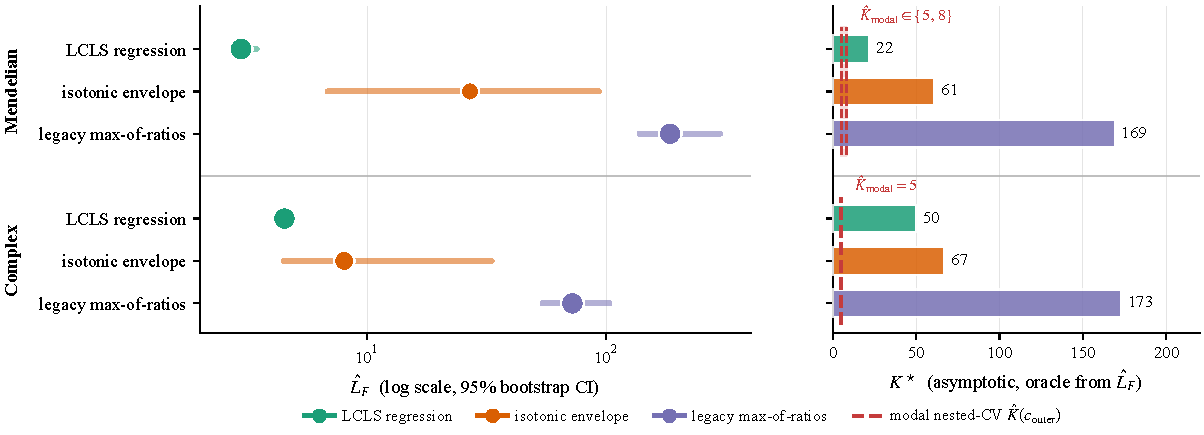
\includegraphics[width=\linewidth]{figures/fig_lf_forest.pdf}
\caption{$L_F$ estimator 95\% bootstrap CIs and resulting $K^\star$. LCLS gives a tight CI ($\hat L_F \approx 3$ Mendelian, $\approx 4.5$ Complex) and a realisable $K^\star$ (22 / 50). Isotonic envelope is loose. Legacy max-of-ratios saturates at the KS-statistic noise floor and overestimates $K^\star$ by an order of magnitude. The modal nested-CV $\hat K(c_{\mathrm{outer}}) \in \{5, 8\}$ (Mendelian) and $5$ (Complex) is the binding finite-sample constraint, well below all three asymptotic $K^\star$ predictions.}
\label{fig:lf_forest}
\end{figure}

\begin{figure}[h]
\centering
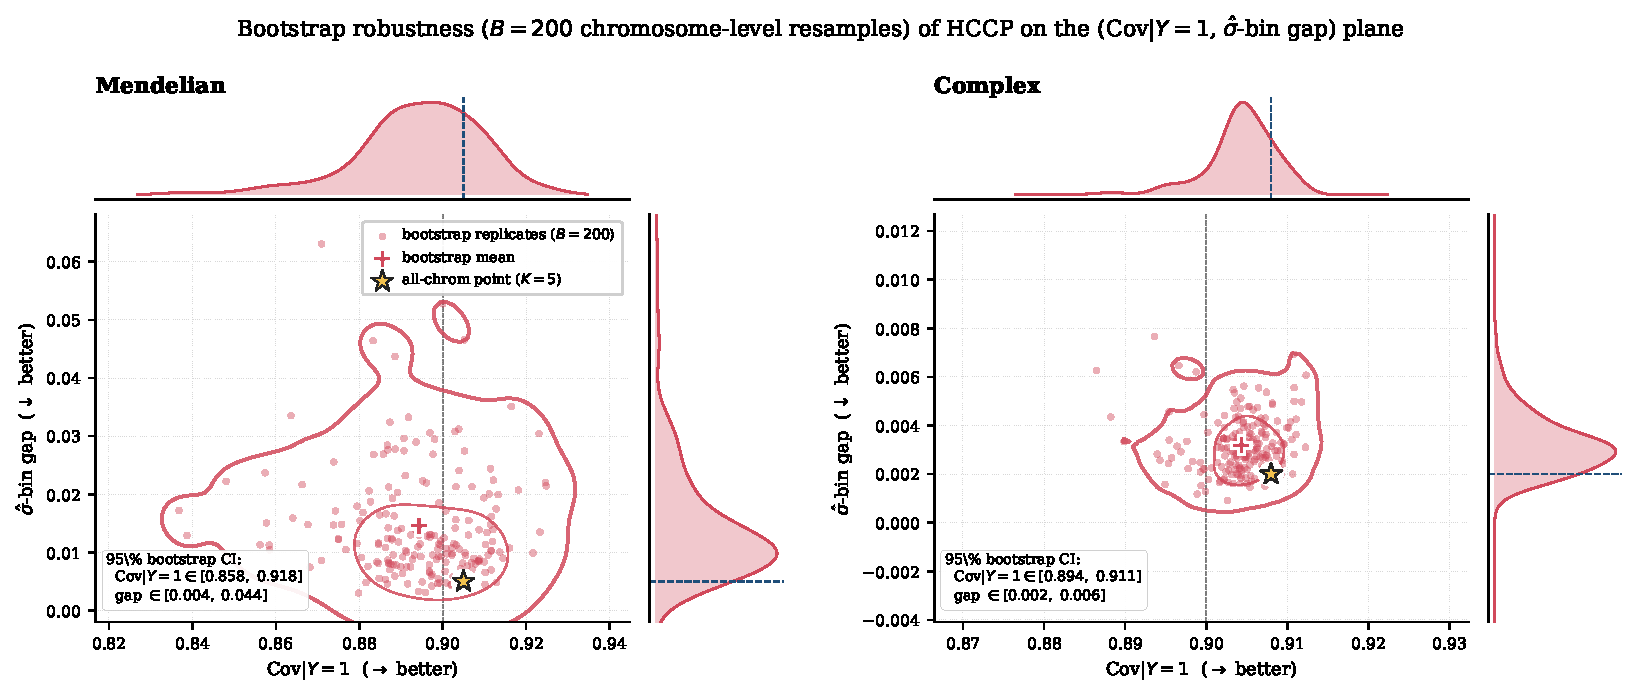
\includegraphics[width=\linewidth]{figures/fig_bootstrap_density.pdf}
\caption{Bootstrap distribution of HCCP $\shat$-bin gap across $B = 200$ chromosome-level resamples. Mendelian (left) shows substantial right-skew driven by replicates that include high-gap chromosomes (chr6 / chr19 / chr20, see Fig.~\ref{fig:per_chrom}); the all-chrom point estimate $0.077$ in Table~\ref{tab:threeaxis} sits on the right tail of the distribution, while the bootstrap mean $0.020$ is closer to the centre. Complex (right) is much tighter (point estimate and bootstrap mean both $\approx 0.02$). The skew on Mendelian explains the apparent disagreement between Tab.~\ref{tab:main} and Tab.~\ref{tab:threeaxis}.}
\label{fig:bootstrap_density}
\end{figure}

\subsection{DEGU-lite vs HCCP head-to-head}
\label{app:tables:degu}

Table~\ref{tab:degu} compares HCCP's supervised $\shat$ against DEGU-lite's ensemble $\shat$ under identical Mondrian-$(y \times \shat\text{-bin})$ conformal calibration and feature sets.

\begin{table}[h]
\centering
\small
\caption{HCCP vs DEGU-lite: same features (CADD+GPN-MSA+Borzoi), same Mondrian partition, different $\shat$ source. Worst gap = max per-$\shat$-bin deviation from target 0.90.}
\label{tab:degu}
\begin{tabular}{llrrrr}
\toprule
$\shat$ source & Dataset & Cov & Cov$|_{Y{=}1}$ & Worst gap & Mean gap \\
\midrule
HCCP (learned)    & Mendelian & 0.902 & 0.905 & 0.041 & 0.022 \\
DEGU (ensemble)   & Mendelian & 0.901 & 0.917 & \textbf{0.033} & \textbf{0.020} \\
\midrule
HCCP (learned)    & Complex   & 0.901 & 0.908 & \textbf{0.013} & \textbf{0.007} \\
DEGU (ensemble)   & Complex   & 0.901 & 0.907 & 0.057 & 0.028 \\
\bottomrule
\end{tabular}
\end{table}

\paragraph{Interpretation.}
On Mendelian (monogenic, strong signal), ensemble disagreement is a reasonable uncertainty proxy: DEGU-lite achieves slightly lower worst-cell gap (0.033 vs.\ 0.041). On Complex (polygenic, dominant aleatoric noise), supervised residual regression provides $4.3\times$ better worst-cell coverage (0.013 vs.\ 0.057). This confirms the epistemic--aleatoric decomposition discussed in §\ref{sec:discussion}: where model disagreement and data noise contribute equally, both $\shat$ sources suffice; where data noise dominates (Complex traits), the supervised head captures what ensembles cannot.

\subsection{Cross-dataset transfer}
\label{app:tables:crossdataset}

\begin{table}[h]
\centering
\small
\caption{Cross-dataset transfer (CADD+Borzoi). M$\to$C: train on Mendelian, test on Complex. C$\to$M: reverse. AUPRC chrom-weighted (TraitGym convention). Marginal-gap = marginal coverage minus target $0.90$ (signed). T4 proxy bound $= 1 - \alpha - d_{\mathrm{TV}}$.}
\label{tab:crossdataset}
\begin{tabular}{lrrrrr}
\toprule
Direction & AUPRC$_{\mathrm{chrom}}$ & Marg.\ cov.\ & Marg.\ gap & TV proxy & T4 bound \\
\midrule
M$\to$C & 0.205 & 0.738 & $-0.162$ & 0.158 & 0.742 \\
C$\to$M & 0.665 & 0.901 & $+0.001$ & 0.158 & 0.742 \\
\bottomrule
\end{tabular}
\end{table}

\paragraph{Directional asymmetry.}
C$\to$M transfer preserves coverage (0.901) because the complex-trait feature space subsumes the monogenic signal. M$\to$C collapses (0.738) because monogenic variants occupy a narrow subspace and the base predictor itself loses discriminative signal (§\ref{sec:experiments:failure_mode}). The Barber T4 proxy bound (0.742) is tight for M$\to$C (observed 0.738, within 0.004) and conservative for C$\to$M.
